MI-EEG信号的采集是一个涉及多层面复杂交互的过程,其间采集的数据易受多种因素交织影响,其中包括但不限于硬件设备性能、受试者个体生理状态以及周围环境条件等变量。这些因素在数据的质量和特性上留下印记,具体体现在诸如通道信号分布的均匀性、伪影的产生与抑制等方面,使得有效解析和后续处理MI-EEG信号成为一项挑战性的工作。

\begin{enumerate}
    \item 通道选择:研究发现,运动想象分类的精度会随着通道数的逐渐增加而提高\cite{chang1998annual},但与此同时,
\end{enumerate}

轻量级:
+scse
+scse 激活函数由sigmoid换为softmax
+sese


eegtrans 等都经过了滤波预处理
在复现实验中效果不好
证明对噪声敏感


自注意力机制由Vaswani等人于2017年提出,是Transformer模型中的一种核心机制\cite{vaswani2017attention},
    其最早应用于自然语言处理领域,此后在计算机视觉等领域也得到了广泛的应用。
    自注意力机制允许神经网络在处理序列数据时,无需考虑输入序列的固定顺序或长度,
    而是通过计算每个位置上的元素与序列中所有其他元素的相关性来动态获取上下文信息,
    相较于其他注意力机制,自注意力机制减少了对外部信息的依赖,更擅长捕捉数据或特征的内部相关性。


    EEGNet\cite{lawhern2018eegnet}是一个用于EEG信号解码的紧凑的端到端网络,其采用了计算机视觉领域的深度卷积和可分离卷积,有效减少了模型的参数量。
EEGNet的结构如图~\ref{fig:EEGNet}所示,其通过三个模块对原始二维输入进行处理:
第一个模块包含时间卷积和空间卷积,其中,时间卷积通过多个卷积核将输入扩展到深度维度,空间卷积采用深度卷积以减少参数的数量;
第二个模块由包含深度卷积和逐点卷积的可分离卷积组成,在减少参数的同时,在深度维度上促进了时空特征的融合;
第三个模块用于分类,将特征直接传入softmax进行分类,从而减少自由参数的数量。
\begin{figure}
  \centering
  \includegraphics[width=\textwidth]{EEGNet.pdf}
  \caption{EEGNet结构}
  \label{fig:EEGNet}
\end{figure}

EEGNet模型简单、参数量小,在设计上借鉴了EEG信号解码领域的经典特征提取算法滤波器组共空间模式(Filter Bank Common Spatial Pattern,FBCSP),
非常适合小数据集的MI-EEG分类任务,是许多相关研究的基础网络。因此,论文以EEGNet为基础,进行下一步的改进。


Inception模块的层次数量和分支数量是影响其性能表现的两项关键参数,论文通过系统实验对这两项指标进行调整。参照文献\cite{santamaria2020eeg},实验中将Inception模块的层级结构分别设定为一层、二层和三层,分别命名为Inception-1、Inception-2和Inception-3。同时,基于实践经验与对EEG信号特征的理解,将分支数目分别设定为3、4和5个,相应地,将具有对应分支数量的Inception模块分别标记为Inception-n3、Inception-n4和Inception-n5,以探究不同层级与分支配置对模型性能的影响。在进行实验时,固定了除待调整参数之外的其他参数,实验结果分别如表~\ref{tab:inception-layer}~和表~\ref{tab:inception-block}~所示。
\begin{table}[ht]
  \centering
  \caption{Inception层次数量实验结果对比}
  \label{tab:inception-layer}
  \begin{tabularx}{\textwidth}{CCC}
    \toprule
    Models & ACC(\%) & Kappa \\
    \midrule
    Inception-1 & \textbf{75.71} & \textbf{0.67} \\
    Inception-2 & 72.57 & 0.63 \\
    Inception-3 & 66.85 & 0.56 \\
    \bottomrule
  \end{tabularx}
\end{table}
\begin{table}[ht]
  \centering
  \caption{Inception分支数量实验结果对比}
  \label{tab:inception-block}
  \begin{tabularx}{\textwidth}{CCC}
    \toprule
    Models & ACC(\%) & Kappa \\
    \midrule
    Inception-n3 & \textbf{72.54} & \textbf{0.63} \\
    Inception-n4 & 71.15 & 0.61 \\
    Inception-n5 & 71.42 & 0.62 \\
    \bottomrule
  \end{tabularx}
\end{table}

实验结果显示,采用单层Inception模块且分支数设定为3时,模型展现出了最优性能。随着Inception模块层数的递增,模型性能呈下降态势,这与之前研究认为浅层网络与特征相对简单的EEG信号更适配的观点相吻合。同时,随着参数规模的增大,过拟合风险也随之增加。

在探究分支数量变化的实验中,对于含3个分支的Inception模块,其特征提取的时间窗口设置为0.1秒、0.3秒和0.5秒,这对应着对4Hz及以上频带的信号特征提取。而对于拥有4个或5个分支的Inception模块,则在此基础上增加了0.7秒和0.9秒的时间窗口,从而进一步涵盖更低频段的特征提取。实验数据显示,随着分支数量增多,模型性能经历了先下降后回升的变化过程。这可能是由于2Hz以上的高频EEG信号(对应0.5秒以内的时间窗口)包含了更为关键的特征信息,虽然多尺度特征提取有助于提升网络性能,但较低频段的特征相对次要,而且,分支数量过多可能加剧过拟合风险,不利于模型的整体性能优化。

目前的大多数迁移都是做二分类 四分类比较少

奈奎斯特-香农(Nyquist–Shannon)采样定理指出,如果一个系统以超过信号最高频率至少两倍的速率对模拟信号进行均匀采样,那么原始模拟信号就能从采样产生的离散值中完全恢复


\begin{table}[ht]
  \centering
  \caption{轻量化卷积模块实验结果对比}
  \label{tab:lite}
  \begin{tabularx}{\textwidth}{CCCC}
    \toprule
    Models & Paramters & FLOPs & ACC(\%) \\
    \midrule
    GAS/SAS(0.5) & 7.31K & 130.37M & 74.61\\
    GAS/SAS(0.4) & 7.83K & 143.44M & 73.80\\
    GAS/SAS(0.6) & \textbf{6.80K} & \textbf{117.75M} & \textbf{74.61}\\
    SG(0.5) & 7.27K & 129.93M & 73.26\\
    SG(0.4) & 7.67K & 139.73M & 72.22\\
    SG(0.6) & 7.27K & 129.93M & 73.00\\
    Origin & 29.99K & 690.37M & \textbf{75.62}\\
    \bottomrule
  \end{tabularx}
\end{table}

\begin{sidewaystable}[ht]
	\caption{HA-FuseNet与其他模型在测试集上的被试内实验结果对比(Acc/SD)}
	\centering
    \label{tab:2acomparein1}
	\begin{tabularx}{\textwidth}{CCCCCCCCCCCC}
        \toprule
        Models & 1 & 2 & 3 & 4 & 5 & 6 & 7 & 8 & 9 & Average & SD \\
        \midrule
        ShallowConvNet \\
        DeepConvNet \\
        EEGNet \\
        EEGConformer \\
        EEGInception \\
        LMDA-Net \\
        \bottomrule
	\end{tabularx}
\end{sidewaystable}


\begin{table}[ht]
  \centering
  \caption{HA-FuseNet与其他模型在测试集上的被试内实验结果对比(Acc)}
  \label{tab:2acomparein}
  \begin{tabularx}{\textwidth}{CCCCCCC}
    \toprule
    Subject & \makecell[c]{Shallow\\ConvNet} & \makecell[c]{Deep\\ConvNet} & EEGNet & \makecell[c]{EEG\\Inception} & \makecell[c]{EEG\\Conformer} & \makecell[c]{HA-\\FuseNet} \\
    \midrule
    1 & 85.07 & 83.68 & 78.13 & 71.18 & 67.71 \\
    2 & 61.46 & 65.28 & 63.54 & 48.26 & 55.21 \\
    3 & 94.10 & 90.63 & 82.30 & 82.29 & 84.72 \\
    4 & 73.26 & 69.44 & 60.42 & 55.90 & 53.82 \\
    5 & 73.26 & 76.04 & 71.88 & 64.58 & 75.69 \\
    6 & 57.29 & 64.58 & 59.03 & 52.43 & 53.47 \\
    7 & 86.81 & 89.93 & 72.92 & 75.00 & 69.10 \\
    8 & 89.93 & 79.51 & 68.06 & 85.41 & 71.53 \\
    9 & 85.42 & 73.61 & 66.67 & 73.61 & 58.68 \\
    \midrule
    Average \\
    SD \\
    \bottomrule
  \end{tabularx}
\end{table}

\begin{table}[ht]
  \centering
  \caption{HA-FuseNet与其他模型在测试集上的被试间实验结果对比(Acc)}
  \label{tab:2acomparecross}
  \begin{tabularx}{\textwidth}{CCCCCC}
    \toprule
    Models & 1 & 2 & 3 & 4 & 5\\
    \midrule
    ShallowConvNet \\
    DeepConvNet \\
    EEGNet \\
    EEGResNet \\
    EEGInception \\
    EEGConformer \\
    LMDA-Net \\
    \midrule 
    HA-FuseNet \\
    \bottomrule
  \end{tabularx}
\end{table}
\begin{table}[ht]
  \centering
  \caption{HA-FuseNet与其他模型在测试集上的被试间实验结果对比(Acc)}
  \label{tab:2acomparecross}
  \begin{tabularx}{\textwidth}{CCCCCC}
    \toprule
    Models & 1 & 2 & 3 & 4 & 5\\
    \midrule
    ShallowConvNet \\
    DeepConvNet \\
    EEGNet \\
    EEGResNet \\
    EEGInception \\
    EEGConformer \\
    LMDA-Net \\
    \midrule 
    HA-FuseNet \\
    \bottomrule
  \end{tabularx}
\end{table}


\begin{table}[ht]
  \centering
  \caption{HA-FuseNet与其他模型在测试集上的被试内实验结果对比(Acc)}
  \label{tab:2acomparein}
  \begin{tabularx}{\textwidth}{CCCCCCC}
    \toprule
    Subject & \makecell[c]{Shallow\\ConvNet} & \makecell[c]{Deep\\ConvNet} & EEGNet & \makecell[c]{EEG\\Inception} & \makecell[c]{EEG\\Conformer} & \makecell[c]{HA-\\FuseNet} \\
    \midrule
    1 & 85.07 & 83.68 & 78.13 & 71.18 & 67.71 \\
    2 & 61.46 & 65.28 & 63.54 & 48.26 & 55.21 \\
    3 & 94.10 & 90.63 & 82.30 & 82.29 & 84.72 \\
    4 & 73.26 & 69.44 & 60.42 & 55.90 & 53.82 \\
    5 & 73.26 & 76.04 & 71.88 & 64.58 & 75.69 \\
    6 & 57.29 & 64.58 & 59.03 & 52.43 & 53.47 \\
    7 & 86.81 & 89.93 & 72.92 & 75.00 & 69.10 \\
    8 & 89.93 & 79.51 & 68.06 & 85.41 & 71.53 \\
    9 & 85.42 & 73.61 & 66.67 & 73.61 & 58.68 \\
    \midrule
    Average \\
    SD \\
    \bottomrule
  \end{tabularx}
\end{table}

\begin{table}[ht]
  \centering
  \caption{HA-FuseNet与其他模型在测试集上的被试内实验结果对比(Acc)}
  \label{tab:2acomparecross}
  \begin{tabularx}{\textwidth}{CCCCCC}
    \toprule
    Models & 1 & 2 & 3 & 4 & 5\\
    \midrule
    ShallowConvNet \\
    DeepConvNet \\
    EEGNet \\
    EEGResNet \\
    EEGInception \\
    EEGConformer \\
    LMDA-Net \\
    \midrule 
    HA-FuseNet \\
    \bottomrule
  \end{tabularx}
\end{table}
\begin{table}[ht]
  \centering
  \caption{HA-FuseNet与其他模型在测试集上的被试内实验结果对比(Acc)}
  \label{tab:2acomparecross1}
  \begin{tabularx}{\textwidth}{CCCCCC}
    \toprule
    Models & 1 & 2 & 3 & 4 & 5\\
    \midrule
    ShallowConvNet \\
    DeepConvNet \\
    EEGNet \\
    EEGResNet \\
    EEGInception \\
    EEGConformer \\
    LMDA-Net \\
    \midrule 
    HA-FuseNet \\
    \bottomrule
  \end{tabularx}
\end{table}


scot-before

首先,通过池化层与卷积层得到Query、Value、Key矩阵,以轴向方式计算空间域的全局自注意力,并通过广播对输入特征图进行加权,随后,进一步计算时空域的全局自注意力,将局部上下文信息引入注意力计算中,提升对特征的表达能力,并对上一步的空间域自注意力进行校准,得到更为丰富且全面的全局时空自注意力表达。将LS-Net


综上所述,尽管运动想象研究已积累了一系列有价值的科研成果,但是依然存在一定的进步空间。
目前基于脑电图的运动想象分类任务仍然存在以下问题:

(1) 当前方法的实施常受限于多种条件,如特征提取依赖于专业神经科学知识与实践经验,对滤波的特定频率范围处理要求严苛,以及需要较高的电极采样密度。然而,在实际应用如家庭级和个性化的运动想象脑机接口系统中,往往不具备专家校验、标准滤波、高时空分辨率、高计算性能等理想条件,导致在实际场景的普适性上存在局限,应用场景较窄。

(2) EEG信号固有的非平稳性和被试特异性导致现有分类方法在不同个体间的性能表现差异较大,即使在部分被试上达到较高识别精度,但在其他被试上可能显著降低,这阻碍了运动想象分类模型在广泛人群中的稳定应用。因此,仍然需要进一步提升分类方法的精确度、稳健性和一致性,从而在各类被试中获得更为满意的表现,取得较为稳定均衡的性能。

(3) 基于深度学习的运动想象脑电图分类模型通常拥有庞大的参数规模,这在计算资源有限的边缘设备上运行效率低下,影响实时响应性能,从而制约了运动想象脑机接口系统的普及推广。因此,有必要研发对模型的参数量进行精简,以实现性能与效率的优化。

(4) EEG数据集因隐私保护、被试生理心理状态变化等因素,普遍具有规模偏小且样本多样性不足的特点。尽管数据增强是应对小规模数据集的有效策略,但针对具有被试特异性的EEG信号,某些增强方法可能破坏原始信号中蕴含的有价值信息。此外,数据增强过程会加重训练阶段的数据处理压力,延长训练周期,对运动想象脑机接口系统的实时响应性能有所制约。因此,如何在有限的小规模数据集上实现高效且稳定的性能提升,是需要考虑的问题。




针对现阶段运动想象脑电图分类任务中仍然存在的问题,论文的研究目标为基于现有方法提出一种改进的新模型,其应当具有以下特点:

(1) 端到端:只进行很少数据预处理的端到端模型,旨在减轻对神经科学先验知识和专家经验的依赖,简化数据处理步骤,降低计算成本,并拓宽模型在不同应用场景下的适用范围。

(2) 提升分类精度与泛化能力:在现有方法的基础上进一步提高分类精度,确保模型能在多样化的被试群体中都展现出优秀且稳定的性能,无论被试个体的特异性如何,都能获得较为理想的分类效果。
%对高空间分辨率、频率滤波无依赖

(3) 轻量化:具有较少的参数规模,使得模型能够在计算资源有限的边缘设备上高效运行,从而提升实时响应性能,促进运动想象脑电图分类技术在实际应用中的部署与普及。

为了实现研究目标,论文基于现有方法进行改进,




为了对模型进行轻量化,论文在SG模块之外,基于ShuffleNetV2提出了GAS/SAS模块。
ShuffleNetV2问题在于,进行Channel Split时,通常是对特征图进行均匀划分,难以灵活调整直传特征图的比例,可能导致对重要特征信息的有效利用率不足。此外,ShuffleNetV2的基础结构在深度维度上的特征变换主要依赖于\(1\times1\)卷积,这在一定程度上限制了其内在的深度特征变换能力。

为了提升ShuffleNetV2基本模块在深度特征变换方面的能力,论文提出了一种可调节分支比例的Shuffle模块(Adaptive Shuffle Module, AS模块),其架构如图~\ref{fig:as}~(a)所示。假设卷积层的输入深度为 \(D_{in}\),输出深度为 \(D_{out}\),针对不同的输入输出深度关系(即 \(D_{in} \le D_{out}\) 和 \(D_{in} > D_{out}\) ),论文对AS模块进行了优化,分别形成了图~\ref{fig:as}~(b)所示的GAS模块(Growing Adjustable Shuffle Module)和图~\ref{fig:as}~(c)所示的SAS模块(Straight Adjustable Shuffle Module)。图中的DW Conv指深度卷积(Depthwise Convolution),\(ratio\)为可调的权重参数。
\begin{figure}
    \centering
    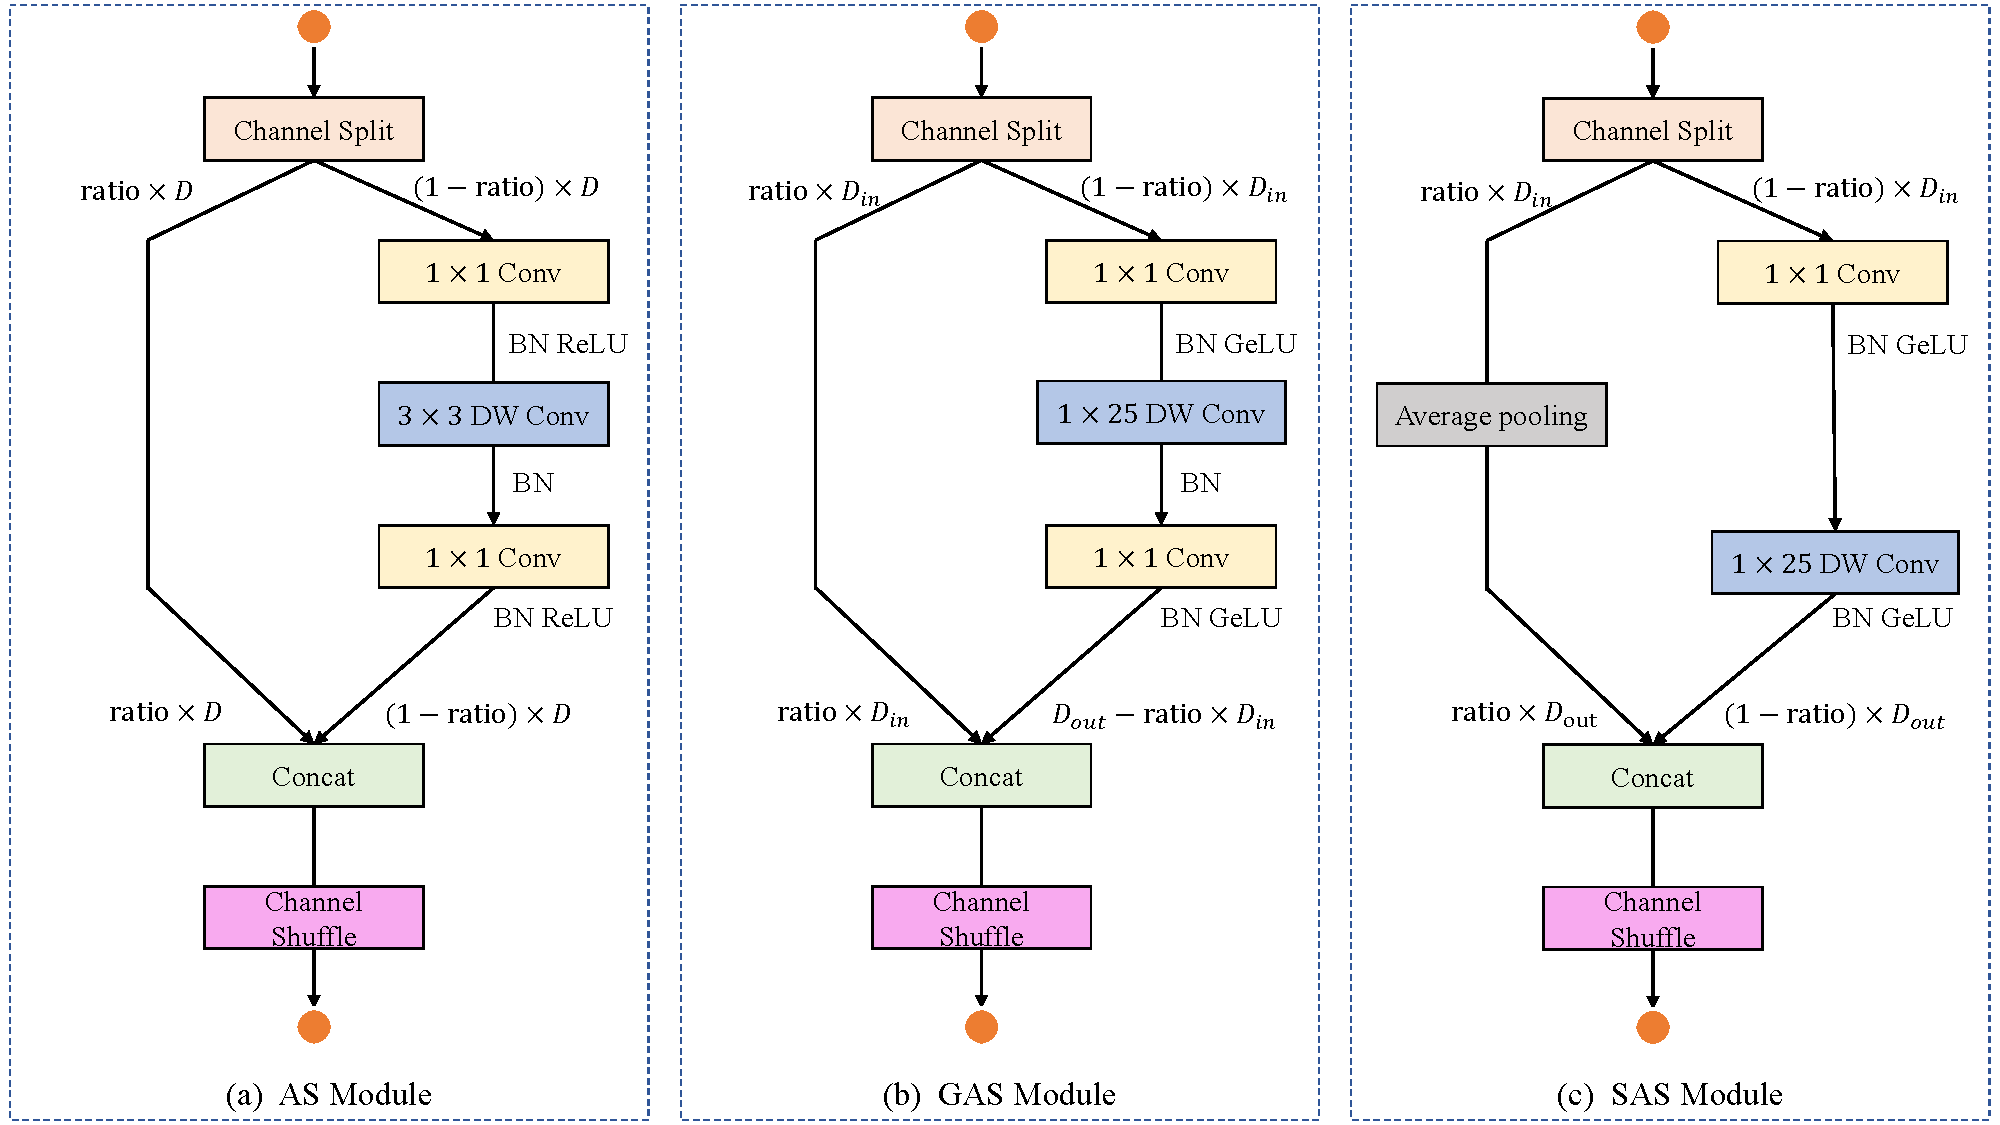
\includegraphics[width=\textwidth]{AS.pdf}
    \caption{AS、GAS、SAS模块结构}
    \label{fig:as}
\end{figure}

对于GAS模块,在保留原有直接传递分支的同时,改动了深度变换的分支的卷积核大小和激活函数,以优化GAS模块对MI-EEG分类任务的性能。对于SAS模块,其在变换分支的设计上采用了与GAS模块一致的改进措施,但去掉了最后的\(1\times1\)卷积层,而由第一个\(1\times1\)卷积层将深度降维至输出维度,再由\(1\times25\)卷积层进行特征的提取。此外,在直接传递分支上,进一步引入了深度维度上的平均池化操作,目的在于在不增添额外参数的前提下,有效减少特征图的数量。相较于原始的Shuffle Unit,GAS模块和SAS模块在功能上进行了扩展,不仅包含了特征维度的升维和降维处理,而且还引入了一个可调节的权重参数 \(ratio\),以动态控制两个分支的特征图数量,从而在处理MI-EEG分类任务时,能够更加灵活和高效地调整特征空间的分布和深度特征的提取。

论文针对通道混洗算法进行了优化升级,使其具备了对不同数量分组及不同数量组内特征图进行灵活、均衡混洗的能力。这使得无论待重排的组及组内特征图的数量如何变化,该算法都能够实现有效的特征交互与信息整合。